\section{Statistical Learning Theory}
STL mainly deals with \textbf{supervised learning} problems: given an input (feature) space $\mathcal{X}$ and an output (label) space $\mathcal{Y}$ (typically $\mathcal{Y} = \{ +1, -1 \}$), the goal is to estimate a functional relationship between the input and output space:

$$
f: \mathcal{X} \xrightarrow{} \mathcal{Y}
$$

Usually, $f$ is called \textbf{classifier}, so a \textbf{classification algorithm} is a procedure that takes the training data ($(X_1, Y_1), .., (X_n, Y_n) \in \mathcal{X} \times \mathcal{Y}$) as input, and provides the classifier $f$ as output.

\subsection{Assumptions}
Moreover, SLT makes the following \textbf{assumptions}:

\begin{enumerate}
    \item There exists a joint probability distribution $P$ among $\mathcal{X} \times \mathcal{Y}$, which is usually not known;
    \item The training examples $(X_i, Y_i)$ are sampled i.i.d. from $P$.
\end{enumerate}

In particular, 

\begin{itemize}
    \item In STL, no assumptions are made on $P$, whereas in \textit{statistical inference} the data are assumed to follow a certain distribution;
    \item The distribution of $P$ is unknown at learning time;
    \item Non-deterministic labels due to label noise or overlapping classes;
    \item The distribution of $P$ is fixed, both during training and testing.
\end{itemize}

\subsection{Losses and risks}
Clearly, we need to have some measure of how good a function $f$ is when used as a classifier, so a \textbf{loss function} measures the "cost" of classifying instance $x \in \mathcal{X}$ as $y \in \mathcal{Y}$. 

In this sense, the simplest loss function is the \textbf{0-1 loss}, which is defined as:

$$
l(X,Y,f(X)) = \begin{cases}
    1 \qquad \text{if } f(X) \neq Y \\
    0 \qquad \text{otherwise}
\end{cases}
$$

We can define the \textbf{theoretical risk} of a function $f$ the average loss over data points generated according to the underlying distribution $P$:

$$
R(f) := \mathbb{E}(l(X,Y,f(X)))
$$

The \textbf{best classifier} is the one with the smallest risk $R(f)$: among all possible classifiers, the best one is the \textit{Bayes classifier}:

$$
f_{\text{Bayes}} := \begin{cases}
    1 \qquad \text{if } P(Y = 1 | X = x) \geq 0.5 \\
    -1 \qquad \text{otherwise}
\end{cases}
$$

Its idea is to classify the most frequent class. However, in practice it is impossible to directly compute the Bayes classifier, since the underlying distribution $P$ is unknown to the learner, and estimating $P$ from the data usually doesn't work.

Recall: Bayes' theorem says that:

$$
P(h|e) = \frac{P(e|h) P(h)}{P(e)} = \frac{P(e|h) P(h)}{P(e|h) P(h) + P(e|\Bar{h}) P(\Bar{h})}
$$
, where:

\begin{itemize}
    \item $P(h)$ represents the \textbf{prior probability} of hypothesis $h$;
    \item $P(h|e)$ represents the \textbf{posterior probability} of $h$ after the evidence $e$;
    \item $P(e|h)$ represents the \textbf{likelihood} of evidence $e$ on hypothesis $h$.
\end{itemize}

Returning to the classification problem, now the situation is that given:

\begin{itemize}
    \item A set of training data $(X_1, Y_1), .., (X_n, Y_n) \in \mathcal{X} \times \mathcal{Y}$ drawn i.i.d. from an \textit{unknown} distribution $P$;
    \item A loss function,
\end{itemize}

the goal is to determine a function $f: \mathcal{X} \to \mathcal{Y}$ which has a risk $R(f)$ which is as close as possible to the risk of the Bayes classifier. However, we notice that it is impossible to compute the risk of $f$ without knowing $P$..

\subsection{The nearest neighbor (NN) rule} A possible solution for this problem could be represented by the \textbf{nearest neighbor} approach, according to which the label of a data point $x$ is given by the label of the nearest point to $x$. Notice that in this case, no assumptions about the probability distribution of the data is used, since the method only uses information from the training set.

But, how good is the NN rule? It was showed that:

$$
R(f_{\text{Bayes}}) \leq R_{\infty} \leq 2R(f_{\text{Bayes}})
$$
, where $R_{\infty}$ denotes the expected error rate of NN when the sample size tends to infinity. Notice that we cannot say anything stronger about the bounds, since there are probability distributions for which the performance of the NN rule achieves either the upper or lower bound.

There exist some variations to the NN rule, for example the \textbf{$k$-NN} rule, which uses $k$ nearest neighbors and takes the majority vote, or the \textbf{$k_n$-NN rule}, which does the same, but for $k_n$ growing with $n$.

\textbf{Theorem (Stone, 1977)}: if $n \to \infty$ and $k \to \infty$, such that $k/n \to 0$ (i.e. $n$ grows faster than $k$), then for all probability distributions, $R(k_n - \text{NN}) \to R(f_\text{Bayes})$, i.e. the $k_n - \text{NN}$ rule is universally Bayes consistent.

However, all these NN rule have some \textbf{disadvantages}:

\begin{itemize}
    \item Not having a learning phase (\textit{lazy algorithm}), a huge amount of data must be kept in memory;
    \item They are very time demanding.
\end{itemize}

\subsection{The kernel rule}
The idea of \textbf{kernel rules} is that rather than fixing the number of neighbors, to classify a new point $x$ we might consider fixing a distance $h$ and taking a majority vote among the labels of all examples that fall within a distance $h$ of $x$. 

\begin{figure}[h!]
		\centering
        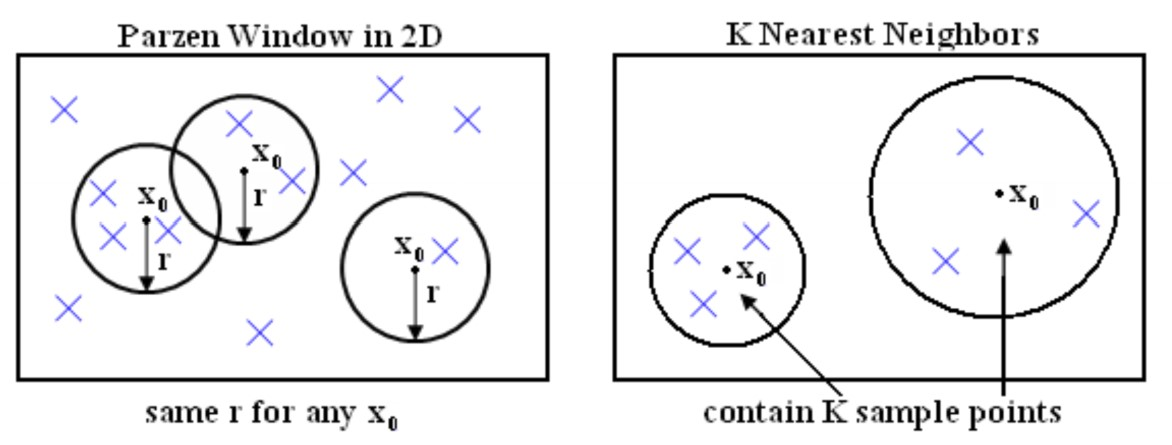
\includegraphics[scale = 1.0]{img/kernel rules.jpg}
		\label{mi}
        \caption{Difference between kernel rules and NN rule}
\end{figure}

Notice that in NN rule, the number of neighbors is fixed, while in kernel rule it depends on the value of $h$. The parameter $h$ is usually called \textbf{smoothing factor} (or \textbf{bandwidth}).

A \textbf{kernel} (a.k.a. \textit{Parzen windows}) is defined as:

$$
K(\Bar{x}) = \begin{cases}
    1 \qquad \text{if } ||\Bar{x}|| \leq 1 \\
    0 \qquad \text{otherwise}
\end{cases}
$$

and we define the vote counts as:

$$
v_n^0(\Bar{x}) = \sum_{i = 1}^n I_{\{ y_i = 0 \}} K \bigleft( \frac{\Bar{x} - \Bar{x}_i}{h} \bigright)
$$

, i.e. the sum of all the elements with label 0 that are within $\Bar{x}$ and $\Bar{x}_i$, and

$$
v_n^1(\Bar{x}) = \sum_{i = 1}^n I_{\{ y_i = 1 \}} K \bigleft( \frac{\Bar{x} - \Bar{x}_i}{h} \bigright)
$$

, i.e. the sum of all the elements with label 1 that are within $\Bar{x}$ and $\Bar{x}_i$.

Then, we assign $x$ to the class 0 if and only if $v_n^0(x) \geq v_n^1(x)$. 

A basic window kernel is represented in Picture \ref{basic kernel}, while Picture \ref{different kernels} shows other possible kernels that can be used.

\begin{figure}[h!]
		\centering
        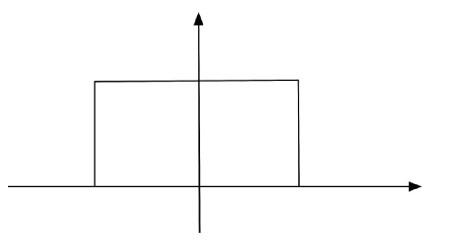
\includegraphics[scale = 1.0]{img/basic window kernel.jpg}
		\label{basic kernel}
        \caption{Basic window kernel}
\end{figure}

\begin{figure}[h!]
		\centering
        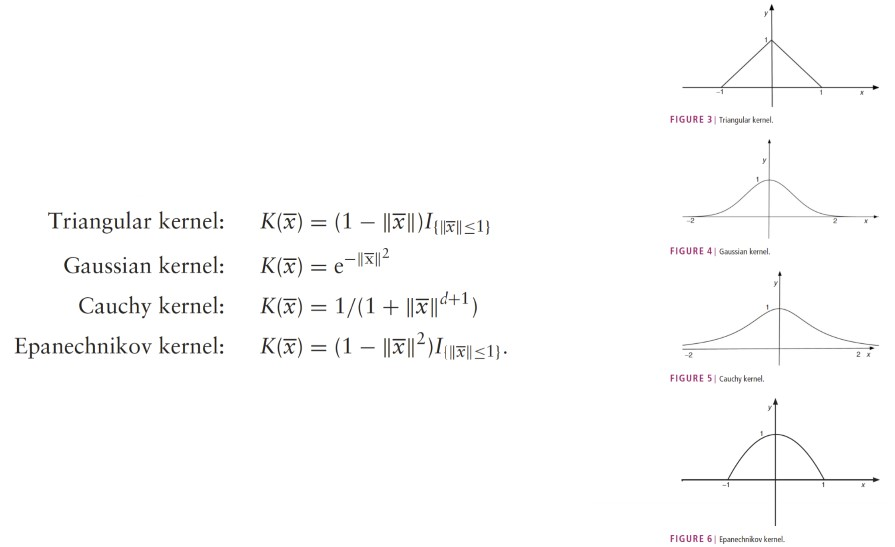
\includegraphics[scale = 1.2]{img/different kernels.jpg}
		\label{different kernels}
        \caption{Other possible kernels}
\end{figure}

\subsection{Empirical Risk Minimization (ERM)}
At the end of 1960's, the \textbf{Empirical Risk Minimization} theory was introduced, and it is based on the following \textbf{principle}: instead of looking for a function which minimizes the true risk $R(f)$, we try to find one which minimizes the \textbf{empirical risk}, i.e. the error the model makes on the training data, which is defined as:

$$
R_{\text{emp}} = \frac{1}{n} \sum_{i = 1}^n l(X_i, Y_i, f(X_i))
$$

Given a training data $(X_1, Y_1), .., (X_n, Y_n) \in \mathcal{X} \times \mathcal{Y}$, a function space $\mathcal{F}$ and a loss function, we define the classifier $f_n$ as:

$$
f_n := \text{arg} \min_{f \in \mathcal{F}} R_{\text{emp}}(f)
$$

, i.e. we choose from $\mathcal{F}$ the function that minimizes the empirical risk. This approach is called the \textbf{empirical risk minimization (ERM)} induction principle, and is motivated from the law of large numbers.

However, we have the issue of how to choose the function space $\mathcal{F}$: a fundamental result in SLT is that the set of rules in $\mathcal{F}$ cannot be too rich, where the richness of $\mathcal{F}$ is measured by its \textbf{VC dimension}.

\subsection{Estimation vs approximation}
Before proceeding, let us introduce a few concepts:
\begin{itemize}
	\item \textbf{Bayes error}: error of the best possible predictor (i.e. the Bayes predictor);
	\item \textbf{Approximation error}: error related to the type of model we are assuming (i.e. related to $\mathcal{F}$). The model may not reflect the nature of the underlying probability distribution. In other words, the approximation error is the minimum generalization error achievable by a predictor in $\mathcal{F}$, and it depends only of $\mathcal{F}$;
	\item \textbf{Estimation error}: error of a predictor belonging to family $\mathcal{F}$. Each predictor in the family will bring an additional error to the approximation error. In other words, the estimation error is the difference between the error of the considered predictor and the error of the predictor, belonging to $\mathcal{F}$, which minimizes the training error (the "best" predictor). The quality of this estimate depends on both the (size of) the training set and on the complexity of the hypothesis class $\mathcal{F}$.
\end{itemize}

Ideally we want to make $R(f_n) - R(f_{Bayes})$ as small as possible, as $n \rightarrow \infty$. Denoting by $f_{\mathcal{ F }}$ the best classifier in $\mathcal{ F }$, the difference can be decomposed as:
$$R \left( f _ { n } \right) - R \left( f _ { B a y e s } \right) = \underbrace{\left( R \left( f _ { n } \right) - R \left( f _ { \mathcal { F } } \right) \right)}_{\text{estimation error}} + \underbrace{\left( R \left( f _ { \mathcal { F } } \right) - R \left( f _ { \text {Bayes} } \right) \right)}_{\text{approximation error}}$$

, where

\begin{itemize}
	\item $R(f_n)$ is the risk of the considered classifier;
	\item $R(f_\mathcal{ F })$ is the risk of the best classifier $f$ on the family $\mathcal{ F }$;
	\item $R \left( f _ { \text {Bayes} } \right)$ is the risk of the best classifier overall (Bayes).
\end{itemize}

\image{img/estimation}{Estimation vs approximation.}{0.35}

According to the complexity of $\mathcal{ F }$ we can have:
\begin{itemize}
	\item \textbf{small complexity} of $\mathcal{ F }$: small estimation error (small \textbf{variance}), large approximation error (large \textbf{bias}), resulting in \textit{underfitting};
	\item \textbf{large complexity} of $\mathcal{ F }$: large estimation error (large \textbf{variance}), small approximation error (small \textbf{bias}), resulting in \textit{overfitting}.
\end{itemize}

The best overall risk is achieved for "moderate" complexity.

\image{img/overunderfitting}{Underfitting vs Overfitting graph}{0.55}
\image{img/modelselection}{Model selection.}{0.8}

\paragraph*{Shattering.} A set of $n$ instances $x_1, \dots, x_n$ from the input space $\mathcal{X}$ is said to be \textit{shattered} by a function class $\mathcal{ F }$ if all the $2^n$ labelings of them can be generated using functions from $\mathcal{ F }$.\\ 
For instance, with $\mathcal{ F }$ as a linear decision functions (straight lines) in the plane, we can have:
\begin{enumerate}[label=(\alph*)]
	\item Any set of 3 non-collinear points shatters $\mathcal{ F }$
	\item No set of 4 points can shatter $\mathcal{ F }$
\end{enumerate}
\imageb{img/shattered}{0.85}

\paragraph*{The Vapnik–Chervonenkis dimension.} The \textbf{VC dimension} of a function class $\mathcal{ F }$, denoted $VC(\mathcal{ F })$, is the largest integer $h$ such that there exists a sample of size $h$ which is shattered by $\mathcal{ F }$. It is a measure of complexity of a function class.\\
If arbitrarily large samples can be shattered, then $VC(\mathcal{ F }) = \infty$.\\
For example:
\begin{itemize}
	\item $\mathcal{ F }$ = linear decision functions in $\mathbb{R}^2 \rightarrow VC(\mathcal{ F }) = 3$
	\item $\mathcal{ F }$ = linear decision functions (hyperplanes) in $\mathbb{R}^n \rightarrow VC(\mathcal{ F }) = n+1$ 
	\item $\mathcal{ F }$ = multi-layer perceptrons with $W$ weights $\rightarrow VC(\mathcal{ F }) = O(W~\log( W))$
	\item $\mathcal{ F }$ = nearest neighbor classifiers $\rightarrow VC(\mathcal{ F }) = \infty$
\end{itemize}


The VC dimension of a classifier depends on the dimension of the space the data points belong to. For instance, if we consider our space to be $\mathbb{R}^2$, then the VC dimension is $3$. As a matter of fact,  $\mathbb{R}^2$ can always shatter any three general position points ("general position" means they do not coincidentally lie on the same line). For instance, consider three points $(0,0)$, $(0,1)$, $(1,0)$. No matter how labels are assigned to them, a line can always separate them. Conversely, let's consider four points $(0,0)$, $(0,1)$, $(1,0)$, $(1,1)$ with label $[+,-,-,+]$, representing the "XOR" function. This function cannot be separated by a line. For $x\in\mathbb{R}$, then the VC dimension is 2 because you cannot separate $+-+$. In general for $x\in\mathbb{R}^d$, the VC dimension for a linear classifier is $d+1$.\\

The \textbf{VC dimension} is usually \textbf{unrelated} to the \textbf{number of free parameters of a model}.\\
For all $f \in \mathcal{ F }$, with probability at least $1-\delta$, we have:
$$
R ( f ) \leq R _ { \mathrm { emp } } ( f ) + \underbrace{\sqrt { \frac { h ( \log ( 2 n / h ) + 1 ) - \log ( \delta / 4 ) } { n } }}_{\text{VC confidence}}
$$
where 

\begin{itemize}
    \item $h=VC(\mathcal{ F })$ is the VC dimension of the family $F$;
    \item $\delta$ is a tolerance parameter;
    \item $n$ is the sample size.
\end{itemize}

We can read this results as:\\

\textit{With probability approaching  1, no matter what the unknown probability distribution, given more and more data, the expected error for the functions that ERM endorses at each stage eventually approaches the minimum value of expected error of the functions in $\mathcal{ F }$ if and only if $\mathcal{ F }$ has finite VC dimension. If VC dimension is equal to $\infty$, like in the KNN case, we have that $R_\text{emp}(f) = 0$ and so $R(f) \leq \infty$ which is meaningless.}\\

Intuitively, since the second term $R_\text{emp}\dots$ is an upper bound, if it is small, $R(f)$ will be small too. This result is fundamental due to the fact that we have no knowledge about $P$, thus we cannot compute $R(f)$, but we can have a \textbf{bound} for it using the second quantity. Indirectly we want to \textbf{reduce the bound} so that at the end the resulting \textbf{risk} is \textbf{minimized}.

\paragraph*{Structural Risk minimization.} It is a general framework for choosing the best classifier. Empirical Risk Minimization only takes care of the \textit{estimation} error (variance) but it is not concerned with the \textbf{approximation error} (bias). The optimal model is found by striking a balance between the empirical risk and the capacity of the function class $\mathcal{ F }$ (ex: the VC dimension).\\
The basic idea of \textit{Structural Risk Minimization} (SRM) is:
\begin{enumerate}
	\item Construct a \textbf{nested} structure for family of function classes $\mathcal{ F }_1 \subset \mathcal{ F }_2 \subset \dots$ with \textbf{non-decreasing VC dimension} $(VC(\mathcal{ F }_1) \leq VC(\mathcal{ F }_2) \leq \dots)$
	\item For \textbf{each class} $\mathcal{ F }_i$, find the solution $f_i$ that \textbf{minimizes} the \textbf{empirical risk}.
	\item Choose the function class $\mathcal{ F }_i$, and the corresponding solution $f_i$ that minimizes the risk bound (= empirical risk + VC confidence) 
\end{enumerate}

Notice that this idea resembles the pruning approach, where we started with a large NN which was trained with back-propagation, and finally reduced. Here the reasoning is the opposite, we start with a small VC dimension and we augment it. 

\image{img/risk_minimization}{Structural risk minimization.}{0.50}